
%%%%%%%%%%%%%%%%% Introduction to the Assignment %%%

In this Assignment, \textit{\textbf{Problem 2 - general radar theory}}, ...


%%%%%%%%%%%%%%%%% TASK 1 %%%
\section{Operational frequency for scientific radar}
The operational frequency for a scientific radar is highly depending on the application and the type of the target. If for example the ionosphere, a so-called soft-target is to be observed, the range resolution of the radar plays a more important role than for example when a hard target is wanted. 


\subsection{Frequency ranges}
According to \todo{add reference ti that oslo presentation} ISR uses frequencies between 50MHz and 2 GHz

3-300mhz csr

Radar stands for \textit{\textbf{Radio Detection and Ranging}}, so Radar generally operates in the RF band, going from about 3MHz to 300GHz \citep{richards2010principles}. Therefore, any of the Radar techniques explained above can be operated in any of those ranges. However, some specific frequency ranges may have advantages and disadvantages for the particular radar technique applied, which is why sometimes ISR, CSR and Doppler Radar Applications are categorized in different bands. Unfortunately, different literature and papers state different ranges, so for example


\subsection{Information gathered by radar measurement}



%%%%%%%%%%%%%%%%% TASK 2 %%%
\section{The radar equation}
To derive the radar equation one starts with the assumption of an isotropic radiation source. Therefore the power density at a distance R is denoted as


\begin{equation}
\label{eq:iso}
	\centering
	Q_{i} = \frac{P_t}{4 \pi R^2} \qquad \bigg[\frac{W}{m^2} \bigg]
\end{equation}

Since usually radar is focused in one specific direction, the equation is multiplied with the Gain G of the antenna

\begin{equation}
\label{eq:dir}
	\centering
	Q_{i} = \frac{P_t G}{4 \pi R^2} \qquad \bigg[\frac{W}{m^2} \bigg]
\end{equation}

When the radiated power now hits a target, a fraction of the power is reflected, or \textit{re-radiated}. This reradiated power is depending on the cross-section $\sigma$ of the hit target. So the received Power density at the antenna is 

\begin{equation}
\label{eq:rePowDen}
	\centering
	Q_{re} = \frac{Q_i \sigma}{4\pi R^2} = \frac{P_t G}{4 \pi R^2} \frac{\sigma}{4\pi R^2} \qquad \bigg[\frac{W}{m^2} \bigg]
\end{equation}

But this received Power is now again dependent on the antenna gain, which is in this case also depending on the antenna effective area $A_{eff}$

\begin{equation}
\label{eq:rePow}
	\centering
	P_{r} = Q_{re} A_{eff} = \frac{P_t G}{4 \pi R^2} \frac{\sigma}{4\pi R^2} A_{eff}\qquad [W]
\end{equation}

The antenna effective area can now be expressed with the help of the antenna gain. The derivation of the gain is not shown here, but it can be derived using the effective area of a Hertzian dipole and the assumption that the antenna perfectly absorbs all received power.\par
This leads to the equation for the antenna effective area, which is depending on the antenna gain and the wavelength $\lambda $ of the used frequency.

\begin{equation}
\label{eq:Aeff}
	\centering
	A_{eff} = G \frac{\lambda^2}{4\pi} \qquad [m^2]
\end{equation}

Inserting this relation in equation \ref{eq:rePow} leads to the so-called Radar Equation, the total received power of the antenna.

\begin{equation}
\label{eq:radEq}
	\centering
	P_{r} = P_t \frac{\rho_a^2 A^2 }{4 \pi \lambda^2 R^2} \sigma \qquad [W]
\end{equation}

where $\rho_{a} $ is the antenna efficiency, defined as

\begin{equation}
\label{eq:effi}
	\centering
	\rho_a = \frac{\lambda^2 G }{4 \pi A} = \frac{A_{eff}}{A}
\end{equation}

with $A$ being the total antenna area.

%%%%%%%%%%%%%%%%% TASK 3 %%%
\section{Cross section calculation}
To calculate the minimum cross section that is detectable for the given values

\begin{center}
\begin{tabular}{c c}
	Object Location & $R$ = 100km \\
	Wavelength & $\lambda$ = 6m \\
	Transmit Power & $P_t$ = 10 kW \\
	Antenna Gain & $G$ = 20 dB = 100 W\\
	System Noise Temperature & $T_s$ = $10^3$ K \\
	Bandwith & $B_w$ = 1 MHz
\end{tabular}
\end{center}

the Signal-to-Noise ratio (SNR) is used. The SNR is the ratio between the received power versus the total system noise Power, where the System Noise Power is, according to \todo{richards zitieren}, denoted as

\begin{equation}
\label{eq:noise}
	\centering
	P_n = N_0 = k_B T_s B_w \qquad [W]
\end{equation}

Using equations \ref{eq:rePow} and \ref{eq:noise}, the SNR can be written as

\begin{equation}
\label{eq:snr}
	\centering
	SNR = \frac{P_r}{P_n} = \frac{P_t G A_{eff} \sigma}{4 \pi R^2 k_B T_s B_w}
\end{equation}

Substituting $A_{eff}$ with eq. \ref{eq:Aeff} and re-ordering \ref{eq:snr} to the cross section area $\sigma$ leads to

\begin{equation}
\label{eq:snr}
	\centering
	\sigma = {SNR} \frac{(4 \pi)^3 R^4 k_B T_s B_w}{P_t G^2 \lambda^2}	\qquad [m^2]
\end{equation}

To calculate the smallest cross section area that is detectable at a range of 100km, one has to assume a minimum SNR, at which the minimum cross section is still detectable.

The minimum SNR, not taking into account LNA's or other instruments to increase the SNR, is obviously 1, since if the signal is stronger than the noise the signal is theoretically detectable.

Inserting $SNR_{min} = 1$ for SNR in eq. \ref{eq:snr} this leads to a minimum cross section

\begin{equation}
\label{eq:crossSecResult}
	\centering
	\sigma_{min} = 0.76105 \qquad [m^2]	
\end{equation}

This is the same result as is given in the assignment sheet.


%%%%%%%%%%%%%%%%% TASK 4 %%%
\section{MST radars}

\subsection{SNR as function of universal time and altitude}
To plot the Signal to Noise ratio as a function of time and altitude, data from 28th of February 2006 is used. The plot can be seen in fig. \ref{img:snrPlot}, the MATLAB Code used to plot these heatmaps can be found in Appendix \ref{code:snr}.

\begin{figure}
	\centering
	\label{img:snrPlot}
	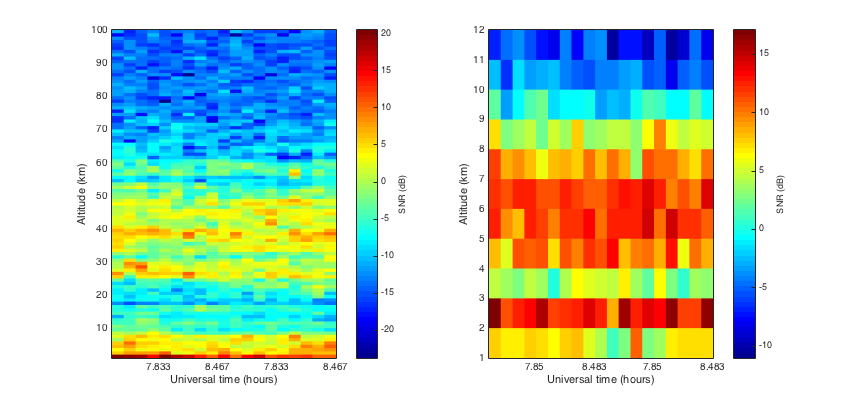
\includegraphics[width=\textwidth]{images/task4_plot1}
	\caption{SNR as function of altitude and time, data from 28Feb06}
\end{figure}


\subsection{Pulse calculations}
To calculate the pulse length, the inter-pulse period (IPP), pulse repetition frequency (PRF )and maximum unambiguous range 	$R_{max}$ for these height resolutions, the following formulas are used:

\begin{center}
\begin{equation}
\centering
\label{eq:pulselength}
	\Delta R = \frac{c \tau_p }{2} \qquad [km] \qquad \textrm{, with } \Delta R \textrm{ as Range resolution and } \tau_p \textrm{ as pulse length}
\end{equation}
\begin{equation}
	{IPP} = \frac{\tau_p }{D} \qquad [s] \qquad \textrm{, with D as duty cycle}
\end{equation}
\begin{equation}
	PRF = \frac{1}{IPP} \qquad [Hz]
\end{equation}
\begin{equation}
\label{eq:rangeMax}
	R_{max} = \frac{c \,  {IPP} }{2} \qquad [km]
\end{equation}
\end{center}

Using these equations the appropriate values for each height resolution is calculated. For the Duty Cycle a value of 5\% is assumed.

\begin{center}
\begin{table}
	\caption{Calculated values using eq. (\ref{eq:pulselength}) to(\ref{eq:rangeMax})}
\begin{center}
\begin{tabular}{ |c | c | c|}
	\hline
	\textbf{Range resolution} & \textbf{150m} & \textbf{1200m} \\
	\hline
	\textbf{Pulse Length} & 1 $\mu s$ & 8 $\mu s$ \\
	\textbf{IPP} & 20 $\mu s$  & 160 $\mu s$ \\
	\textbf{PRF} & 50 kHz & 6250 Hz\\
	\textbf{ R$_{max}$} & 3 km & 24 km\\
	\hline	
\end{tabular}
\end{center}
\end{table}
\end{center}


\subsection{Transmitted pulse length and received signal strength}

\subsection{Atmospheric parameters}